% Synchronized to r43697
\subsection{OPT\_IGMPPROXY - Proxy pour Internet Group Management Protocol}
\configlabel{OPT\_IGMPPROXY}{OPTIGMPPROXY}

Depuis quelques années Telekom AG Allemand utilise le VDSL 25/50 (bande passante~:
25/50 Mbit/s) pour envoyer des paquets de divertissement. Ainsi, il est possible
de recevoir la télévision par Internet (IPTV).

La distribution de la télévision sur IP est effectuée en utilisant le multicast
(ou la multidiffusion), à savoir, un émetteur source unique vers un groupe (fermé).
Pour l'organisation de la diffusion de groupe le protocole réseau IGMP (Internet Group
Management Protocol) est nécessaire. L'IGMP 
(\altlink{http://fr.wikipedia.org/wiki/Internet_Group_Management_Protocol})
offre la possibilité de gérer dynamiquement des groupes multicast. L'administration
ne se trouve pas dans la station d'émission, mais dans le routeur sur lequelle les
destinataires du groupe multicast sont connectés directement. L'IGMP fournit des
fonctions par lesquelles une station notifie au routeur qu'il peut recevoir des paquets
IP multicast pour un groupe multicast particulier.

Les routeurs Speedport (actuellement W700V/W701V/W722) fournissent un support IGMP. Au
lieu d'utiliser des routeurs Speedport, vous pouvez utiliser fli4l avec le support IPTV,
pour cela vous devez installer le proxy IGMP sur le routeur fli4l.

La documentation du paquetage OPT\_IGMP décrit la configuration de fli4l avec une connexion
VDSL et IPTV, vous devez avoir un décodeur (ou STB) X300T/X301T ou MR-303 derrière le routeur
fli4l pour fonctionner. Dans cette documentation, on utilise une carte supplémentaire pour
l'installation de l'IPTV via le réseau.

\subsubsection{Condition préalable}

Telekom VDSL Allemand est présenté comme un VLAN. Dans la phase de lancement (démarrage du
réseau) un seul lien VLAN (ID7) a été utilisé, sur lequel tout le trafic circulait.
Après des modifications (sur le réseau) deux liens VLAN (ID7, ID8) sont utilisés, le lien ID7
reste pour le trafic Internet et le nouveau lien ID8 est utilisé exclusivement pour le trafic
du multicast IPTV. Actuellement les modifications du VDSL pour le réseau (deux liens VLAN ID7/ID8)
sont en grande partie terminées.

Hardware (avec un Set-Top-Box (ou boîtier décodeur) et un modem-VDSL)~:
\begin{itemize}
   \item{Hardware pour fli4l~: avec un VDSL 25/50 vous pouvez utiliser un processeur 486. Si vous
   avez des problèmes avec l'image/son le matériel utilisé est trop faible.}
   \item{Carte réseau haut de gamme (par exemple: 3Com, Intel PRO100). Le chipset Realtek
   est à mon avis un composant bas de gamme}
\end{itemize}

Software~:
\begin{itemize}
   \item{Paquetage~: advanced\_networking}
   \item{Paquetage~: dhcp\_client (pour le réseau et l'utilisation du lien ID8)}
\end{itemize}

La configuration des fichiers de (base.txt, dsl.txt, advanced\_networking.txt, dhcp\_client.txt,
dns\_dhcp.txt) sont décrites dans ce manuel.

\subsubsection{Configutation du hardware}

Recommandation avec le routeur Speedport et une connexion au boîtier décodeur IPTV directement
sur le routeur sans autres éléments dans le réseau, bien sûr, cela s'applique également à fli4l.
Néanmoins, si un n\oe{}ud est interposés (comme un concentrateur, commutateur, pont, passerelle,
routeur) entre le boîtier IPTV et le routeur, il doit être compatible avec le multicast, pour
éviter les interférences.

Le commutateurs (ou switche) est en général pas utilisé dans le réseau domestique, le réseau
virtuel (VLAN) sert à soulager le trafic avec le lien (ID7) et le lien (ID8) pour le trafic
multicast de l'IPTV.

Vous pouvez aussi, pour la configuration du hardware de fli4l utiliser des cartes réseaux séparés
(une carte d'interface réseau = LAN ou carte Ethernet) et une carte pour la connexion du boitier
décodeur pour le trafic multicast, cela soulagera le reste de votre réseau domestique et écartera
les problèmes par rapport à la configuration ci-dessus. Pour ceux qui préfèrent la méthode avec
une 'simple' carte réseau, ils doivent savoir se qu'ils font (car elle n'est pas décrite ici).

Voici deux schémas un avec le routeur par défaut et un avec 3 cartes réseaux installées dans
le routeur fli4l~:

\begin{itemize}
   \item{Configuration par défaut~:
         \begin{itemize}
            \item{La carte réseau eth0 est configurée dans base.txt pour le LAN interne de la maison/bureau.}
            \item{La carte réseau eth1 est configurée dans dsl.txt pour l'interface DSL.}
         \end{itemize}
         \begin{figure}[ht!]
         \centering
         \fontfamily{phv}\selectfont
		 ~~~~~~~Modem-VDSL~~~~~Router-fli4l~~~~~~~~~~~~~~~~\\
         
\includegraphics[]{image001}\\
         ~~~~~~~~~~~~~~~~~~~~~~~~~~~~~~~~~~~~~~~~~~~~Interface-LAN
         \caption{fli4l avec la configuration par défaut}
         \label{fig:standardconfig}
         \end{figure}
      }
   \item{Configuration avancée avec une carte réseau pour l'IPTV~:
         \begin{itemize}
            \item{Après l'installation d'une carte réseau supplémentaire dans le routeur fli4l,
			vous devez configurer la carte supplémentaire eth2 dans base.txt}
         \end{itemize}
         \begin{figure}[ht!]
         \centering
         \fontfamily{phv}\selectfont
		 ~~~~~~~Modem-VDSL~~~~~Router-fli4l~~~~~Interface pour le décodeur IPTV\\
         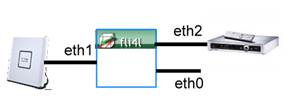
\includegraphics[]{image002}\\
         ~~~~~~~~~~~~~~~~~~~~~~~~~~~~~~~~~~~~~~~~~~~~Interface-LAN
         \caption{fli4l avec la configuration IPTV}
         \label{fig:iptvconfig}
         \end{figure}
      }
\end{itemize}

\subsubsection{Configuration du VLAN}

Tout d'abord~: l'OPT\_IGMP ne dépend pas du VLAN. Le VLAN est plutôt utilisé par Deutsche
Telekom pour le VDSL et doit être supporté par le routeur. Si le VLAN est nécessaire pour
d'autres fournisseurs Internet (Arcor, Alice, etc ..), la configuration est actuelle au-delà
de mes connaissances.

Pour que Internet fonctionne avec le VDSL 25/50 de T-Home, la carte réseau qui est connectée
au modem VDSL doit être configuré comme une interface VLAN.

\vspace{3mm}
\emph{Une note pour ceux qui ont seulement le 'DSL normal', c'est à dire ADSL, ADSL2,
	ADSL2+~: le VLAN est nécessaire uniquement avec le VDSL, mais pas avec le 'DSL normal'.
	La configuration du VLAN ne doit pas être installé avec l'utilisation du 'DSL normal'.}
\vspace{3mm}

Si vous utilisez deux lien VLAN (voir ci-dessus) le trafic se répartit comme ceci~:

\begin{itemize}
   \item{VLAN ID7~: Trafic-Internet}
   \item{VLAN ID8~: Trafic-IPTV Multicast}
\end{itemize}

Donc, le trafic Internet fonctionne indépendamment du trafic IPTV. La principale différence,
il est nécessaire d'utiliser le VLAN ID7 pour les accès entrant PPPoE. Le VLAN ID8 est fournie
par un serveur DHCP sans accès entrant. Dans cette architecture, il n'y a pas de redémarrage
forcé après 24 heures.\\ 

Pour le VLAN la configuration suivante est requise (la carte réseau est indiquée à la section
configuration du matériel)~:\\

\noindent \textbf{advanced\_networking.txt}

\begin{example}
\begin{verbatim}
VLAN_DEV_N='2'
VLAN_DEV_1_DEV='eth1’     # interface of VDSL-Modem; example: eth1
                          # in our example 'eth1' connects to the VDSL modem
VLAN_DEV_1_VID='7         # ID7 to support VLAN for internet
VLAN_DEV_2_DEV='eth1’     # interface of VDSL modem; example: eth1
VLAN_DEV_2_VID='8’        # ID8 to support VLAN for IPTV
\end{verbatim}
\end{example}

\noindent La carte réseau virtual eth1.7 doit être paramétré dans le fichier de configuration DSL~:\\

\noindent \textbf{dsl.txt}

\begin{example}
\begin{verbatim}
PPPOE_ETH='eth1.7'        # eth<number of the card connecting the vdsl modem>.7'
                          # i.e. 'eth1.7'
\end{verbatim}
\end{example}

\noindent Pour la carte réseau virtual eth1.8 vous aurez besoin d'un client\_dhcp, car le VLAN ID8
est configuré par un serveur DHCP sans accès entrant.\\

\noindent \textbf{dhcp\_client}

\begin{example}
\begin{verbatim}
OPT_DHCP_CLIENT='yes'
DHCP_CLIENT_TYPE='dhcpcd'
DHCP_CLIENT_INTERFACES='IP_NET_3_DEV' # listen on interface eth1.8
DHCP_CLIENT_USEPEERDNS='no'
DHCP_CLIENT_HOSTNAME=''
\end{verbatim}
\end{example}

Depuis la v3.3 de fli4l, on ne peut plus définir l'interface avec cette valeur \texttt{eth1.8},
mais vous devez utiliser \texttt{IP\_NET\_x\_DEV} pour définir l'interface depuis le fichier
base.txt; Ici \texttt{IP\_NET\_3\_DEV}.\\

\noindent Facultatif~:\\
Si la carte réseau que vous utilisez a des problèmes avec la taille du MTU, vous pouvez là régler
dans la variable DEV\_MTU. Pendant les testes, la carte Intel Pro/100 (e100) et la 3-Com ont montrées
aucun problème, d'autres utilisateurs ont signalés des problème avec la carte 3Com '3c59x', ils ont
modifiés la valeur MTU à 1496.

\begin{example}
\begin{verbatim}
DEV_MTU_1=''              # Adjust MTU size of NIC on VDSL-Modem
                          # Example: DEV_MTU_1='eth1 1496'
\end{verbatim}
\end{example}

Les fichiers de configuration base.txt et dns\_dhcp.txt doivent être modifiées, comme décrit dans
le chapitre suivant.\\

\subsubsection{Configuration de la carte réseau supplémentaire pour l'IPTV}

Vous devez configuré base.txt et dns\_dhcp.txt pour paramétrer la deuxième carte réseau et le VLAN.\\

\noindent Paramètrage de la deuxième carte réseau pour l'IPTV~:\\

\begin{example}
\begin{verbatim}
NET_DRV_N='2'
NET_DRV_1='via-rhine'     # 1. NIC interface for LAN
NET_DRV_2='3c59x'         # 2. NIC – here 3Com for IPTV SetTopBox
\end{verbatim}
\end{example}

Maintenant nous devons spécifier la plage d'adressage pour la deuxième carte réseau. Nous allons utiliser
pour le réseau local 192.168.2.0/24 et 192.168.3.0/24 pour la deuxième carte réseau. Nous avons besoin
également de paramétrer les cartes virtuelle pour eth1.7 et eth1.8~:\\

\begin{example}
\begin{verbatim}
IP_NET_N='4'
IP_NET_1='192.168.2.1/24'           # home/office LAN
IP_NET_1_DEV='eth0'
IP_NET_2='192.168.3.1/24'           # iptv LAN
IP_NET_2_DEV='eth2'
IP_NET_3='dhcp'                     # dhcp client - IP via dhclient
IP_NET_3_DEV='eth1.8'
IP_NET_3_MAC='00:40:63:da:cf:32'    # new MAC (not the MAC of eth1)
IP_NET_4='dhcp'                     # eth1.7 connecting to the modem
IP_NET_4_DEV='eth1.7'
IP_NET_4_MAC='00:40:63:da:cf:33'    # new MAC (not the MAC of eth1)
\end{verbatim}
\end{example}

Il est important de changer les adresses MAC pour eth1.7 et eth1.8, elles ne doivent pas coïncider
avec eth1, sinon - selon le réseau VDSL - il peut éventuellement se produire des perturbations
après la déconnexion forcée.

Pour que la nouvelle carte réseau puisse accéder à Internet, bien sûr, tout comme pour la première
carte réseau. Ces paramètres supplémentaires sont nécessaires~: \\

\begin{example}
\begin{verbatim}
PF_INPUT_1='IP_NET_1 ACCEPT'
PF_INPUT_2='IP_NET_2 ACCEPT'
PF_INPUT_3='any 224.0.0.0/4 ACCEPT'
[...]
PF_FORWARD_3='any 224.0.0.0/4 ACCEPT'
PF_FORWARD_5='IP_NET_1 ACCEPT'
PF_FORWARD_6='IP_NET_2 ACCEPT'
[...]
PF_POSTROUTING_1='IP_NET_1 MASQUERADE'
PF_POSTROUTING_2='IP_NET_2 MASQUERADE'
\end{verbatim}
\end{example}

Pour que cela fonctionne vous devez paramétrez l'adressage DHCP dynamique sur la carte réseau IPTV,
pour  accéder à la Set-Top Box (ou décodeur) et lui donner un nom. Les paramètres suivants dans
le dns\_dhcp.txt sont nécessaires~: \\

\begin{example}
\begin{verbatim}
HOST_10_NAME='igmp'
HOST_10_IP4='192.168.3.1'
HOST_11_NAME='iptv'
HOST_11_IP4='192.168.3.4'
HOST_11_MAC='00:D0:E0:93:49:34'         # MAC Adr T-Home X300T
[...]
DHCP_RANGE_2_NET='IP_NET_2'
DNSDHCP_RANGE_2_START='192.168.3.10'
DNSDHCP_RANGE_2_END='192.168.3.20'
DNSDHCP_RANGE_2_DNS_SERVER1=''
DNSDHCP_RANGE_2_DNS_SERVER2=''
DNSDHCP_RANGE_2_NTP_SERVER=''
DNSDHCP_RANGE_2_GATEWAY=''
\end{verbatim}
\end{example}

Après avoir configuré la nouvelle carte réseau, il est judicieux de tester l'accès Internet
avec un PC connecté au routeur. Si vous arrivez à vous connecté, la seconde carte réseau sera
configuré correctement.

\subsubsection{Fonctions de l'IGMP}

Lors du démarrage du routeur fli4l les paramètres du fichier de configuration proxy.txt sont
écrit dans le fichier /etc/igmpproxy.conf, ils sont ensuite lu lors du démarrage du proxy IGMP.

Contrairement aux versions antérieures le paquetage opt\_igmp est lancé au démarrage, il est
exécute aussi longtemps que la connexion Internet physique est disponible. Le proxy IGMP n'est
pas affectée par la déconnexion forcé après 24 heures ou par la connexion/déconnexion manuel
de l'accés Internet.

\subsubsection{Configuration de l'IGMP}

\begin{description}

\config{OPT\_IGMPPROXY}{OPT\_IGMPPROXY}{}

Si vous indiquez \var{'yes'}, vous activez le proxy IGMP. avec \var{'no'} vous déactivez
l'ensemble du paquetage.

\config{IGMPPROXY\_DEBUG}{IGMPPROXY\_DEBUG}{IGMPPROXYDEBUG}

Si vous indiquez \var{'yes'} les messages du proxy IGMP sont envoyés à syslog.

\config{IGMPPROXY\_DEBUG2}{IGMPPROXY\_DEBUG2}{IGMPPROXYDEBUG2}

Si vous indiquez \var{'yes'} vous pouvez augmenter le niveau des messages du proxy IGMP.

\config{IGMPPROXY\_QUICKLEAVE\_ON}{IGMPPROXY\_QUICKLEAVE\_ON}{IGMPPROXYQUICKLEAVEON}

Avec Quickleave vous pouvez abaisser la charge de la liaison montante. Si vous avez indiqué
\var{'yes'}, le multicast sera arrêté plus rapidement après un changement de canal et la charge
de la liaison décendante sera réduite par le proxy IGMP, il se comporte comme un récepteur.

Si vous utilisez deux décodeurs et qu'il sont sur le même canal, il peut arriver (avec
l'activation de Quickleave) que le programme soit interrompu sur l'un des décodeurs, vous
devez alors changer le programme. Si vous utilisez un seule décodeur Quickleave peut être
activé en toute sécurité.

\begin{example}
\begin{verbatim}
IGMPPROXY_QUICKLEAVE_ON='yes'      # activate Quickleave mode
                                   # yes or no; Default: yes
\end{verbatim}
\end{example}

\config{IGMPPROXY\_UPLOAD\_DEV}{IGMPPROXY\_UPLOAD\_DEV}{IGMPPROXYUPLOADDEV}

Pour le fonctionnement de l'IPTV avec le proxy IGMP vous avez besoin d'une interface avec
une liaison montante et décendante. L'interface de la liaison montante est l'interface de
la carte réseau qui sera connecté au modem VDSL. Normalement cela doit toujours être la même.

Le transfert de l'IPTV doit se faire sur le lien ID8 avec eth1.8, au lieu de ppp0. Cela doit
être paramétré dans le fichier de configuration.

\begin{example}
\begin{verbatim}
IGMPPROXY_UPLOAD_DEV='eth1.8'      # Upstream interface; Default: ppp0
                                   # eth1.8 for T-Home/VDSL with id7/id8
\end{verbatim}
\end{example}

\config{IGMPPROXY\_DOWNLOAD\_DEV}{IGMPPROXY\_DOWNLOAD\_DEV}{IGMPPROXYDOWNLOADDEV}

L'interface de la liaison décendante (carte réseau pour le décodeur de l'IPTV) dépend de la
configuration matériel. Dans fli4l la deuxième carte réseau eth2 est l'interface pour le décodeur.

\begin{example}
\begin{verbatim}
IGMPPROXY_DOWNLOAD_DEV='eth2'      # Downstream Interface
\end{verbatim}
\end{example}

\config{IGMPPROXY\_ALT\_N}{IGMPPROXY\_ALT\_N}{IGMPPROXYALTN}

Dans cette variable vous indiquez le nombre de plages d'adresse IP pour le flux multicast.

\config{IGMPPROXY\_ALT\_x\_NET}{IGMPPROXY\_ALT\_x\_NET}{IGMPPROXYALTxNET}

Dans la variable IGMPPROXY\_ALT\_NET vous indiquez les adresses IP pour le trafic multicast
provenant de extérieur pour le réseau local, ainsi que l'adresse IP local du décodeur.

\begin{example}
\begin{verbatim}
IGMPPROXY_ALT_N='3'                        # Number of Multicast sources
IGMPPROXY_ALT_1_NET='239.35.0.0/16'        # IPTV streams - always needed
IGMPPROXY_ALT_2_NET='217.0.119.0/24'       # needed for T-Home
IGMPPROXY_ALT_3_NET='193.158.34.0/23'      # needed for T-Home
                                           # before May 2013 '193.158.35.0/24'
# IGMPPROXY_ALT_4_NET='192.168.3.0/24'     # Address range IPTV SetTop-Box/not
                                           # needed anymore
\end{verbatim}
\end{example}

\config{IGMPPROXY\_WLIST\_N}{IGMPPROXY\_WLIST\_N}{IGMPPROXYWLISTN}

Dans cette variable vous indiquez le nombre de listes blanches pour le rapport IGMP.

\config{IGMPPROXY\_WLIST\_x\_NET}{IGMPPROXY\_WLIST\_x\_NET}{IGMPPROXYWLISTxNET}:\newline

Si vous utilisez IGMPv3 toutes les adresses sont regroupées dans un rapport,
(\altlink{http://grinch.itg-em.de/entertain/artikel/zielnetzarchitektur-und-igmpproxy/}). 
Ces adresses seront ensuite complètement ignorées. Cela conduira à un arrêt complet
de tout le trafic multicast par l'émetteur IGMP, en supposant qu'ils ne sont plus
nécessaires. Pour éviter cela, la configuration de listes blanches est utilisée.
Seuls les groupes multicast de cette liste seront épargnés par le WAN.

\begin{example}
\begin{verbatim}
IGMPPROXY_WLIST_N='1'                          # Number of Multicast sources
IGMPPROXY_WLIST_1_NET='239.35.0.0/16'         # IPTV streams - always needed
                                               # see above
\end{verbatim}
\end{example}

\end{description}

\subsubsection{Modification des autres fichiers de configuration}

Avec la révision 32955 il n'est pas nécessaire de paramétrer les règles du pare-feu
pour le proxy IGMP et pour le fux multicast si les règles standard
(\var{PF\_INPUT\_ACCEPT\_DEF='yes'} et \var{PF\_FORWARD\_ACCEPT\_DEF='yes'})
sont activés dans le fichier base.txt, le script de démarrage ajoutera automatiquement
ces règles si la variable \var{OPT\_IGMPPROXY='yes'} est activée.

Il y a deux règles qui sont ajouté dans la chaîne INPUT pour permettre aux messages
entrants d'atteindre le proxy IGMP~:

\begin{example}
\begin{verbatim}
Chain INPUT (policy DROP 0 packets, 0 bytes)
 pkts bytes target   prot opt in   out   source         destination
 [...]
    0     0 ACCEPT   all  --  *    *     0.0.0.0/0      224.0.0.1     \
    /* automatically added for IGMP Proxy */

    0     0 ACCEPT   all  --  *    *     0.0.0.0/0      224.0.0.22    \
    /* automatically added for IGMP Proxy */
 [...]
\end{verbatim}
\end{example}

Vous avez aussi une règle dans la chaîne FORWARD qui permet de transmettre le flux
multicast entrant vers le récepteur de média~:

\begin{example}
\begin{verbatim}
Chain FORWARD (policy DROP 0 packets, 0 bytes)
 pkts bytes target   prot opt in   out   source         destination         
 [...]
    0     0 ACCEPT   all  --  *    *     0.0.0.0/0      239.35.0.0/16  \
    /* automatically added for IPTV streams */
 [..]
\end{verbatim}
\end{example}

Si l'une des règles par défaut n'est pas activée, vous devez au moins paramétrer
et insérer manuellement les règles suivantes.

\begin{example}
\begin{verbatim}
PF_INPUT_x='any 224.0.0.1/32 ACCEPT'
PF_INPUT_x='any 224.0.0.22/32 ACCEPT'
[...]
PF_FORWARD_x='any 239.35.0.0/16 ACCEPT'
\end{verbatim}
\end{example}

\achtung{Remarque~: contrairement aux versions précédentes de la documentation,
	les règles réellement nécessaires ont été écrite pour un réseau limité. Si
	l'IPTV ne fonctionne pas, n'hésitez pas à fournir des informations supplémentaires
	concernant le réseau que vous utilisez.}

\achtung{Important~!
Depuis la fin du mois de mai 2013, Telekom a introduit de nouvelles routes (sans classe prédéfini) pour
améliorer le service (\altlink{http://www.onlinekosten.de/forum/showthread.php?t=116415&page=38}).
Cela est une bonne chose, car plus de 256 émetteurs ou adresses sont utilisables. Maintenant
le serveur DHCP transfére les routes, elles ne sont plus inclusent dans le sous-réseau comme
précédamment. Tant que Telekom ne change pas son sous-réseau du serveur-IPTV (193.158.34.0/23)
la route statique peut être définie vers l'interface vlan8, vous devez faire attention au changement
de celle-ci, sinon le multicast ne fonctionnera plus.}

Solution~: Dans le fichier base.txt, vous devez spécifier une route supplémentaire.

\begin{example}
\begin{verbatim}
IP_ROUTE_N='1'
IP_ROUTE_1='193.158.34.0/23 eth1.8'
\end{verbatim}
\end{example}
